%%%%%%
%
% $Autor: Wings $
% $Datum: 2020-01-18 11:15:45Z $
% $Pfad: githubtemplate/Template/Presentations/Template/slides/rename.tex $
% $Version: 4620 $
%
%
% !TeX encoding = utf8
% !TeX root = Rename
%
%%%%%%



\Mysection{Sensoren und Aktoren}

\STANDARD{Sensoren}
{ 
	
  \framesubtitle{Einleitung}	
  \textbf{Grundsätzlich:} Sensor (lat: \glqq Fühler" ) dienen zur \textbf{qualitativen} und \textbf{quantitaiven Auffassung} von physikalischen, chemischen, biologischen, klimatischen und medizinischen Größen. \cite{Hering:2023} \\ 
  Jedes Sensorsystem besteht aus folgenden Komponenten: 
  \begin{itemize}
  	\item \textbf{Sensor-Element} z.B. veränderlicher Widerstand
  	\item \textbf{Auswerte-Elektronik} z.B. Mikrokontroller
  \end{itemize}
}

\STANDARD{Funktionsprinzip}
{ 
	\textbf{Grundsätzlich:} Wandlung einer \textbf{nicht elektrischen Eingangsgröße} in ein \textbf{elektrisches Ausgangssignal}. \cite{Hering:2023}
\begin{center}
\begin{figure}
\usetikzlibrary{arrows.meta, positioning}
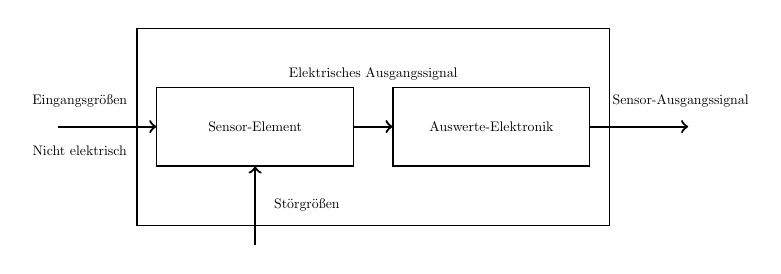
\begin{tikzpicture}[
	scale=0.5,
	transform shape,
	block/.style={draw, rectangle, minimum width=5cm, minimum height=2cm, align=center},
	outer/.style={draw, rectangle, minimum width=12cm, minimum height=5cm},
	arrow/.style={->, thick}
	]
	
	% Outer box
	\node[outer] (system) {};
	
	% Inner blocks
	\node[block] (sensor) at (-3,0) {Sensor-Element};
	\node[block] (eval) at (3,0) {Auswerte-Elektronik};
	
	% Input arrow
	\draw[arrow] (-8,0) -- (sensor.west)
	node[midway, above, xshift=-20pt, yshift=10pt] {Eingangsgrößen}
	node[midway, below, xshift=-20pt, yshift=-10pt] {Nicht elektrisch};
	
	% Between blocks
	\draw[arrow] (sensor.east) -- (eval.west)
	node[midway, above, yshift=30pt] {Elektrisches Ausgangssignal};
	
	% Output arrow
	\draw[arrow] (eval.east) -- (8,0)
	node[midway, above, xshift=30pt, yshift=10pt] {Sensor-Ausgangssignal};
	
	% Disturbance arrow
	\draw[arrow] (-3,-3) -- (sensor.south)
	node[midway, right, xshift=10pt] {Störgrößen};
	
\end{tikzpicture}
	\caption{Wirkprinzip eines Sensorsystemes}
\end{figure}	
	\end{center}
	\textbf{Achtung:} äußere Störgrößen können Einfluss nehmen und müssen daher berücksichtigt werden (z.B. Berücksichtigung der Temperaturabhängigkeit)
}
\STANDARD{Lichtschranken} 



\STANDARD{Optische Näherungssenoren}
{ 
Optische Näherungssensoren nutzen Sensorelemente, welche sowohl aus \textbf{Transmitter} als auch aus \textbf{Receiver} bestehen. Hierbei sind \textbf{Strahlenquellen} beispielsweise der \textbf{Sender} und \textbf{Fotodioden} die \textbf{Empfänger}. 
\begin{itemize}
	
	\item \textbf{Einweg-Lichtschranken:} Sender und Empfänger gegenüberliegend. Hohe Auflösung, bis zu 10m \cite{Hering:2023}
	\item \textbf{Reflex-Lichtschranken:} Sender und Empfänger in einem Gehäuse, \textbf{Reflektor}. Einfache Einstellung, bis zu 5m Abstand \cite{Hering:2023}
\end{itemize}
}
\STANDARD{Optische Näherungssenoren}
{ 
	\begin{center}
	\begin{figure} 
	\usetikzlibrary{arrows.meta, positioning}
	
\usetikzlibrary{arrows.meta, positioning}

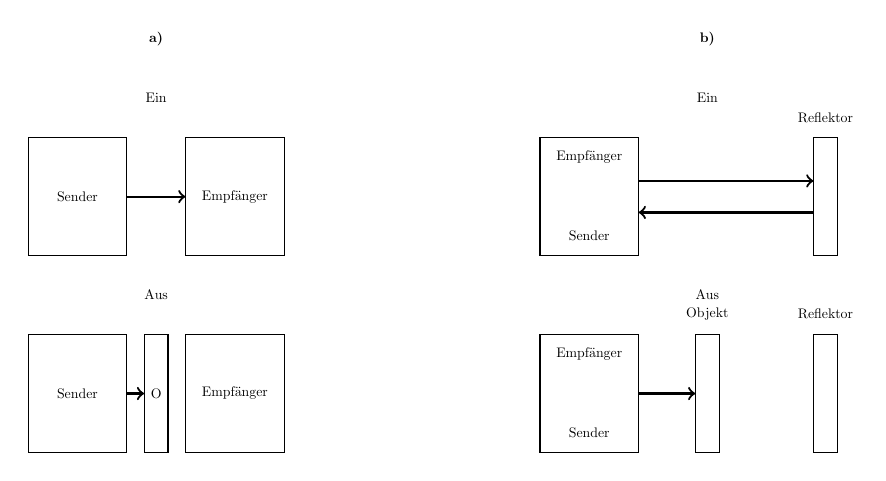
\begin{tikzpicture}[
	scale=0.50,
	transform shape,
	block/.style={draw, rectangle, minimum width=2.5cm, minimum height=3cm, align=center},
	smallblock/.style={draw, rectangle, minimum width=0.6cm, minimum height=3cm},
	arrow/.style={->, thick},
	label/.style={font=\normalsize}
	]
	
	% ======================
	% a) Einweglichtschranke
	% ======================
	\node[label] at (-8,6) {\textbf{a)}};
	
	% EIN (oben)
	\node[label] at (-8,4.5) {Ein};
	
	\node[block] (S1) at (-10,2) {Sender};
	\node[block] (E1) at (-6,2) {Empfänger};
	
	\draw[arrow] (S1.east) -- (E1.west);
	
	% AUS (unten)
	\node[label] at (-8,-0.5) {Aus};
	
	\node[block] (S2) at (-10,-3) {Sender};
	\node[smallblock] (O) at (-8,-3) {};
	\node[block] (E2) at (-6,-3) {Empfänger};
	
	\draw[arrow] (S2.east) -- (O.west);
	
	\node at (O.center) {O};
	
	% ======================
	% b) Reflektorlichtschranke
	% ======================
	\node[label] at (6,6) {\textbf{b)}};
	
	% EIN (oben)
	\node[label] at (6,4.5) {Ein};
	
	\node[block] (SE1) at (3,2) {};
	\node[smallblock] (R1) at (9,2) {};
	
	% Beschriftungen exakt ausgerichtet
	\node[label] at (3,3) {Empfänger};
	\node[label] at (3,1) {Sender};
	\node[label] at (9,4) {Reflektor};
	
	% Hin- und Rückstrahl symmetrisch
	\draw[arrow] ([yshift=0.4cm]SE1.east) -- ([yshift=0.4cm]R1.west);
	\draw[arrow] ([yshift=-0.4cm]R1.west) -- ([yshift=-0.4cm]SE1.east);
	
	% AUS (unten)
	\node[label] at (6,-0.5) {Aus};
	
	\node[block] (SE2) at (3,-3) {};
	\node[smallblock] (OBJ) at (6,-3) {};
	\node[smallblock] (R2) at (9,-3) {};
	
	\node[label] at (3,-2) {Empfänger};
	\node[label] at (3,-4) {Sender};
	\node[label, yshift=15pt] at (6,-1.5) {Objekt};
	\node[label, yshift=15pt] at (9,-1.5) {Reflektor};
	
	\draw[arrow] (SE2.east) -- (OBJ.west);
	
\end{tikzpicture}
\caption{a) Einweg-Lichtschranke, b) Reflex-Lichtschranke}
	\end{figure}
	\end{center}
}

\STANDARD{LED}
{
	\begin{center}
		\begin{figure}
			
			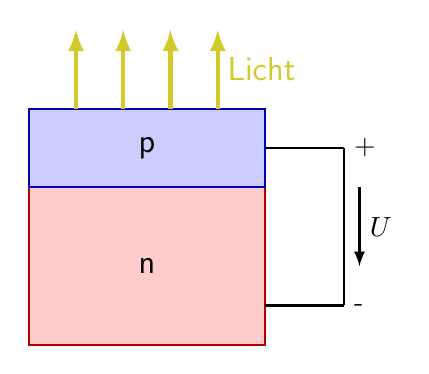
\begin{tikzpicture}[>=latex, font=\sffamily]
				
				% --- n-Schicht ---
				\fill[red!20] (0,0) rectangle (3,2);
				\draw[thick, red!70!black] (0,0) rectangle (3,2);
				\node at (1.5,1) {\large n};
				
				% --- p-Schicht ---
				\fill[blue!20] (0,2) rectangle (3,3);
				\draw[thick, blue!70!black] (0,2) rectangle (3,3);
				\node at (1.5,2.5) {\large p};
				
				% --- Lichteinfall (nun von unten nach oben gedreht) ---
				\foreach \x in {0.6,1.2,1.8,2.4}{
					\draw[->, ultra thick, yellow!80!black] (\x,3) -- (\x,4);
				}
				\node[yellow!80!black, right] at (2.4,3.5) {\large Licht};
				
				% --- Elektrischer Anschluss ---
				% Pluspol oben
				\draw[thick] (3,2.5) -- (4,2.5) node[right] {+};
				\draw[thick] (3,0.5) -- (4,0.5) node[right] {-};
				
				% Verbindung und Spannungspfeil
				\draw[thick] (4,2.5) -- (4,0.5);
				\draw[->, thick] (4.2,2) -- (4.2,1) node[midway, right] {$U$};
				
			\end{tikzpicture}
			\caption{Funktionsprinzip einer LED \cite{Walker:2014}}
		\end{figure}
	\end{center}




}



\STANDARD{Funktionsprinzip Fotodiode}
{\begin{center}
		\begin{figure}
			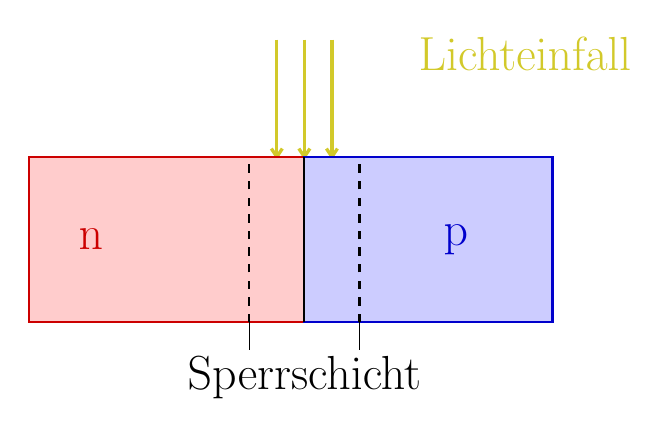
\begin{tikzpicture}[scale=0.7]
				
				% Stil für alle Knoten
				\tikzset{every node/.style={font=\fontsize{18.2pt}{23.7pt}\selectfont}}
				
				% Lichteinfall (gelb)
				\foreach \x in {10.5,11,11.5} {
					\draw[very thick, yellow!80!black] (\x,15.5) -- (\x,13.375);
					% kleine Querstriche am Ende
					\draw[very thick, yellow!80!black] (\x,13.375) -- ++(-0.1,0.15);
					\draw[very thick, yellow!80!black] (\x,13.375) -- ++(0.1,0.15);
				}
				\node[text=yellow!80!black] at (15,15.25) {Lichteinfall};
				
				% n-Schicht (rot)
				\filldraw[fill=red!20, draw=red!80!black, thick]
				(6,10.375) rectangle (11,13.375);
				\node[text=red!80!black] at (7.125,11.875) {n};
				
				% p-Schicht (blau)
				\filldraw[fill=blue!20, draw=blue!80!black, thick]
				(11,10.375) rectangle (15.5,13.375);
				\node[text=blue!80!black] at (13.75,11.875) {p};
				
				% Sperrschicht
				\draw[dashed, thick, black!70!black] (10,10.375) -- (10,13.375);
				\draw[dashed, thick, black!70!black] (12,10.375) -- (12,13.375);
				\draw[thick] (11,10.375) -- (11,13.375);
				\node at (11,9.375) {Sperrschicht};
				
				% kleine Linien unten
				\draw (10,9.875) -- (10,10.375);
				\draw (12,9.875) -- (12,10.375);
				
			\end{tikzpicture}
			\caption{Funktionsprinzip Fotodiode \cite{Walker:2014}}
		\end{figure}
	\end{center}
	
}


\STANDARD{ Aktor Funktionsprinzip } 
{
\textbf{Fazit:} 
\begin{itemize}
	\item \textbf{Sender (LED):} Durch \textbf{Stromfluss} werden Photonen emittiert. 
	\item \textbf{Empfänger (Fotodiode):} Durch \textbf{Lichteinfall} wird ein Stromfluss erzeugt. 

	\end{itemize}

}
\STANDARD{\textbf{Der SENSOR VON UNS HIER }}
{ \begin{center}
		
	
	\end{center}
}

\STANDARD{Aktoren}
{ 
\textbf{Grundsätzlich:} Aktoren dienen der \textbf{Erzeugung} von \textbf{Bewegungen} oder der Aufbringung von \textbf{Kräften} und \textbf{Momenten}. Hierbei fasst der Begriff alle Ausgabeelemente die sowohl analog (z.B. Stellmotoren)  als auch binär (z.B. Relais ) wirken können zusammen \cite{Roddeck:2023} 
}

\STANDARD{Motoren}
{ 
\textbf{Grundsätzlich:} Durch das \textbf{Bestromen} einer \textbf{Spule} wird gegenüber einem \textbf{bestehenden Magnetfeld (Permanent- oder Elektromagnet)} eine Kraft aufgebracht, welche dann in einem \textbf{Moment} resultiert. \cite{Feynman:2020} 
\begin{itemize}
	\item \textbf{Moment $\propto$ Stromstärke} 
	\item \textbf{Drehzahl $\propto$ Spannung }
\end{itemize}

}




%Durch \textbf{Rotation eines Magnetfeldes)} wird ein \textbf{Anzugsmoment} auf den rotierenden Körper (\textbf{\glqq Rotor"}) erzeugt. Hierbei \textbf{muss} das \textbf{äußere Magnetfeld schneller} rotieren als der \textbf{Rotor} selbst. \cite{Feynman:2020}



\STANDARD{Motortreiber}
{ 
	
	
	
}

\STANDARD{Möglichkeiten der Steuerung }
{ 
	
	
	
}



\begin{frame}[fragile]{Code}

%, numbers=left, caption={Konstruktion eines Keras-Sequential-Modells}, label={src:kerasmodel}]

  \begin{lstlisting}[language=Python]
import tensorflow as tf
from tensorflow.keras import datasets, layers, models

MODEL = models.Sequential()
  \end{lstlisting}

\end{frame}

\begin{frame}[fragile]{Code}

  \lstinputlisting[language=Python, firstnumber=1]{Code/PDFExtractTable/PDFExtractTable.py}
\end{frame}
